\chapter{Methodology}

\section{Data Collection}
\paragraph{ }The data used in this study was collected from \ac{TIMBER} with the help of Dr. Gianluca Valentino who has access to the \acs{CERN} Intranet. Data was collected from the instrumentation discussed in Section \ref{sec::beam_instrumentation} and covers 1624 Injections over a time period of 3 months (from 17\textsuperscript{th} August to 20\textsuperscript{th} October 2018). During this time, approximately 65 experiments were performed.

\paragraph{ }The file sizes for the data gathered from each instrument ranged from 4 KB to 2 MB, these were initially individually analysed (refer to Section \ref{sec::Data_Cleaning_and_Analysis}) and then merged to create the dataset used to run the anomaly detection algorithms on (refer to Section \ref{sec::Merging_the_Dataset}). The total size of the merged datasets were 231 KB and 324 KB for Beam 1 and Beam 2 respectively. Loading this data in memory was not an issue since the file size is rather small, thus the problem of dealing with Big Data was not encountered in this study.

\section{Data Cleaning and Analysis}
\label{sec::Data_Cleaning_and_Analysis}
\paragraph{ }After Data Extraction, the provided datasets were analysed separately in order to understand their nature, remove any outliers and be able to aggregate the data correctly for further analysis. In this section the results of this analysis will be presented with the hopes that the reader will have a more clear understanding of later results. Note that all the steps mentioned here were repeated for both beams.

\subsection{\acs{TDI} \acs{BLM}s}
\paragraph{ }There are three \acs{BLM}s in the \acs{TDI}, each one giving 10 readings around the moment of injection. In order to get a total loss for each injection, the sum of each reading from the 3 monitors was taken (\ref{fig::TDI_BLM_hist}). From the plot of this data (Figure \ref{fig::Raw_TDI_BLM}) it was noted that at the exact moment of injection, there was a spike in the amount of beam lost. Thus, in order to then obtain a single reading corresponding to that particular injection, the maximum sum of losses for each 10 second window was kept. 

\begin{figure}[!t]
	\begin{minipage}[b]{0.475\linewidth}
		\centering
		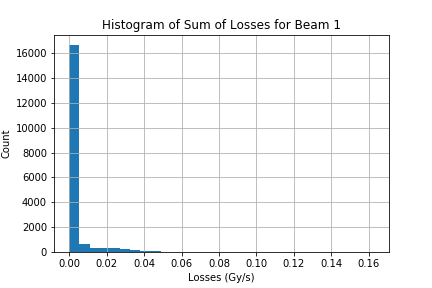
\includegraphics[width=\textwidth]{Histogram_of_Sum_of_Beam_Losses}
		\caption[BLM Histogram]{Histogram of Sum of Losses for Beam 1}
		\label{fig::TDI_BLM_hist}
	\end{minipage}	
	\hspace{0.25cm}
	\begin{minipage}[b]{0.475\linewidth}
		\centering
		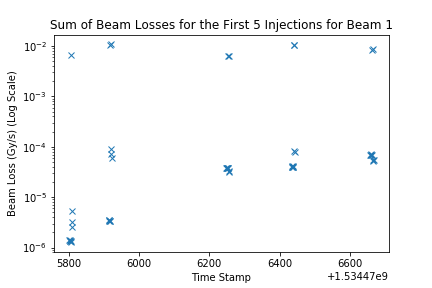
\includegraphics[width=\textwidth]{Raw_Beam_Loss}
		\caption[BLM Time Series]{Time Series of Beam Loss Sum for the First 5 Injections}
		\label{fig::Raw_TDI_BLM}
	\end{minipage}	
\end{figure}

\begin{figure}[b]
	\centering
	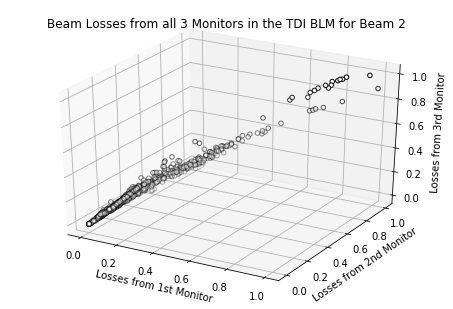
\includegraphics[width=0.6\textwidth]{BLM_3D_Plot}
	\caption[BLM Correlation Plot]{Beam Losses from all 3 Monitors in the TDI BLM for Beam 2 after MinMax Scaling}
	\label{fig::TDI_BLM_3D}
\end{figure}  

\paragraph{ }Once the relevant readings were kept, the sum column was dropped and this data set was saved to be used for anomaly detection. Furthermore, after scaling these points using MinMax scaling, it was noted from Figure \ref{fig::TDI_BLM_3D} that the readings from the 3 monitors are highly correlated. This was confirmed by computing the correlation matrix which gave a Pearson Correlation value $> 0.98$ for all pairwise comparisons.

\subsection{Abort Gap}
\paragraph{ }Similar to the \acs{TDI} \acs{BLM} readings, the Abort Gap readings also come in groups of 10 readings around the moment of injection. In this case however, the change in Abort Gap population is of interest for this study, thus the difference between every 10\textsuperscript{th} reading was kept and saved to be used for anomaly detection.

\begin{figure}[!t]
	\begin{minipage}[b]{0.475\linewidth}
		\centering
		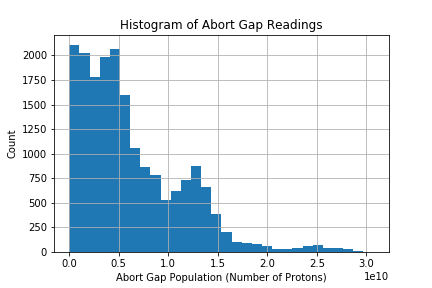
\includegraphics[width=\textwidth]{Histogram_of_Abort_Gap_Population}
		\caption[Abort Gap Histogram]{Histogram of Abort Gap Population for Beam 1}
		\label{fig::Abort_Gap_hist}
	\end{minipage}	
	\hspace{0.25cm}
	\begin{minipage}[b]{0.475\linewidth}
		\centering
		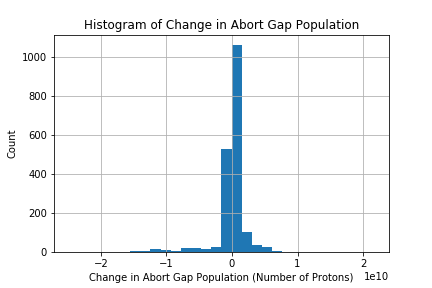
\includegraphics[width=\textwidth]{Histogram_of_Change_in_Abort_Gap_Population}
		\caption[Change in Abort Gap Histogram]{Histogram of Change in Abort Gap Population for Beam 1}
		\label{fig::Change_in_Abort_Gap_hist}
	\end{minipage}	
\end{figure}

\begin{figure}[b]
	\centering
	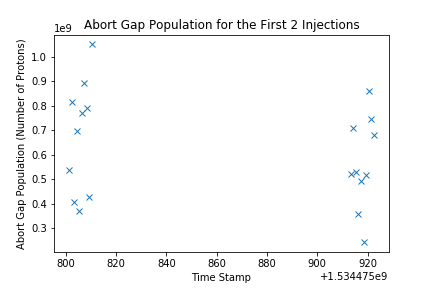
\includegraphics[width=0.6\textwidth]{Time_Series_of_Abort_Gap_Population}
	\caption[Abort Gap Time Series]{Time Series of Abort Gap  Population for the First 8 Injections}
	\label{fig::Abort_Gap_Time_Series}
\end{figure}  


\paragraph{ }Figures \ref{fig::Abort_Gap_hist} and \ref{fig::Change_in_Abort_Gap_hist} show the histograms of the Abort Gap Population and the Change in Abort Gap Population respectively. A time series plot of the Abort Gap Readings can be seen in Figure \ref{fig::Abort_Gap_Time_Series}.

\subsection{SPS and LHC Intensities}

\section{Feature Selection}


\section{Merging the Dataset}
\label{sec::Merging_the_Dataset}